\documentclass[12pt, french]{article}

\usepackage{fancyhdr, fancybox, lastpage}
\usepackage[most]{tcolorbox}
\usepackage[a4paper, margin={0.3in, .75in}]{geometry}
\usepackage{wrapfig}
\usepackage[version=4]{mhchem}

\pagestyle{fancy}
\renewcommand\headrulewidth{1pt}
\renewcommand\footrulewidth{1pt}
\fancyhf{}
\rhead{ \em{Zakaria Haouzan}}
\lhead[C]{\em{2ème année baccalauréat Sciences physiques}}
\chead[C]{}
\rfoot[C]{}
\lfoot[R]{}
\cfoot[]{\em{Page \thepage / \pageref{LastPage}}}


\newtcolorbox{Box2}[2][]{
                lower separated=false,
                colback=white,
colframe=white!20!black,fonttitle=\bfseries,
colbacktitle=white!30!gray,
coltitle=black,
enhanced,
attach boxed title to top left={yshift=-0.1in,xshift=0.15in},
title=#2,#1}


\begin{document}
\begin{center}
   \shadowbox {\bf{Suivi temporel d’une transformation - Vitesse de réaction }}
\end{center}

\vspace{-0.2cm}
%%_________________________Exercice ! :"_________________________Exercice
   \begin{Box2}{Exercice 1 :(SN2024)  Suivi temporel d’une transformation}
     \begin{wrapfigure}[9]{r}{0.4\textwidth}
  \begin{center}
	  \vspace{-0.6cm}
	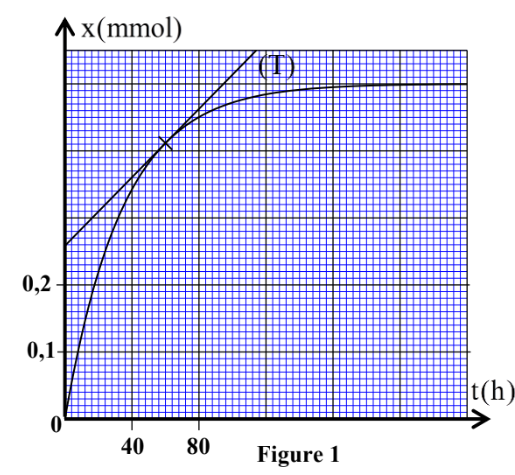
\includegraphics[width=0.4\textwidth]{./img/suivi_01.png}
  \end{center}
\end{wrapfigure}

     \emph{
L'acide ascorbique, de formule brute $C_6H_8O_6$
appelé vitamine C, est un antioxydant présent dans de
nombreux fruits et légumes. La vitamine C possède des propriétés rédox et
     acido-basiques. Cette vitamine se }dégrade à la chaleur, à l’air ;... 

On se propose d’étudier dans cet exercice :
\begin{itemize}
  \item le suivi temporel de la dégradation de la vitamine C dans un jus d'orange,
  \item le dosage d’une solution aqueuse contenant de la vitamine C.
\end{itemize}
     \subsection*{Partie 1 : Suivi temporel de la dégradation de la vitamine C dans un jus d'orange}
On dispose d’une solution (S) de jus d'orange de volume $V=200mL$ à une température $\theta$. Si on expose ce
jus à l’air, la vitamine C qu’il contient se dégrade par oxydation avec le dioxygène.
On suit, par dosage, l’évolution temporelle de la dégradation de cette vitamine. Le graphe de la figure1
représente l’évolution temporelle de l’avancement x de la réaction d’oxydation de la vitamine C. La droite
(T) dans la figure 1 représente la tangente à la courbe au point d’abscisse $t = t_1 = 60h$.

\begin{enumerate}
  \item Répondre par vrai ou faux (sans justification) aux
affirmations suivantes : (0,75 pt)
\begin{enumerate}
  \item La concentration initiale des réactifs est un facteur cinétique.
  \item L’évolution d’un système chimique est toujours considérée
comme terminée au bout d’une durée égale à deux fois le temps
de demi-réaction.
\item Plus les chocs entre les espèces réactives sont nombreux et
efficaces, plus la réaction chimique est rapide.
\end{enumerate}
\item Déterminer graphiquement $t_{1/2}$ le temps de demi-réaction. (0,5pt)
\item Déterminer, en unité $mmol.L^{-1}.h^{-1}$, la vitesse volumique de la réaction à l’instant $t_1$ . (1pt)
\end{enumerate}
   \end{Box2}


%%_________________________Exercice !2 :"_________________________Exercice
\begin{Box2}{Exercice 2 : (SN2021)Etude cinétique d’une réaction chimique}
%\begin{wrapfigure}{r}{0.22\textwidth}
  %\begin{center}
	  %\vspace{-0.6cm}
	%\includegraphics[width=0.22\textwidth]{./img/Ex2.png}
  %\end{center}
%\end{wrapfigure}
L’une des plus anciennes réactions de synthèse est la fabrication du savon. Le savon est un produit
composé de molécules obtenues par réaction chimique, entre un composé organique et une solution
aqueuse d'hydroxyde de sodium.

Cette partie de l’exercice se propose d’étudier, par conductimétrie, la cinétique de la réaction de
synthèse d’un savon. Cette réaction se produit entre l’éthanoate d’éthyle de formule
  $CH_3COOC_2H_5$ et une solution aqueuse d’hydroxyde de sodium $Na_{(aq)}^{+} + HO^-_{(aq)}$

  À un instant choisi comme origine des dates t = 0, on introduit, en excès, l’éthanoate d’éthyle dans un
ballon contenant une quantité de matière $n_0(HO^-) = 10^{-3} mol$ d’ions hydroxyde. On obtient un
mélange réactionnel ayant un volume $V_0 = 100mL$.

Il se produit, sous une température constante, une réaction modélisée par l’équation chimique
  suivante :  \ce{CH3COOC2H5_{(aq)} + HO^-_{(aq)} -> CH3COO^-_{(aq)} + C2H5OH_{(aq)}}

\end{Box2}


%%_________________________Exercice ! 3:"_________________________Exercice
\begin{Box2}{Exercice 2 : (SN2021)Etude cinétique d’une réaction chimique }
\begin{wrapfigure}{r}{0.4\textwidth}
  \begin{center}
	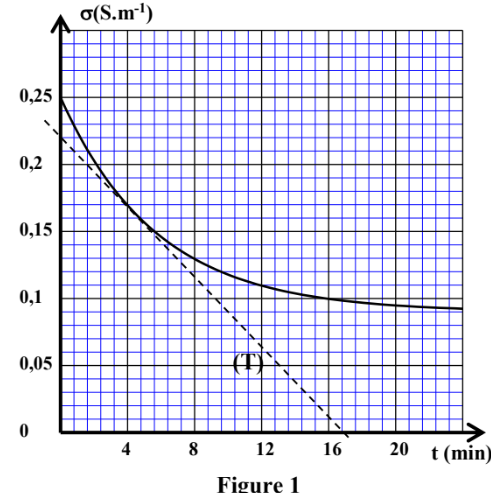
\includegraphics[width=0.4\textwidth]{./img/suivi_02.png}
  \end{center}
\end{wrapfigure}


  \textbf{1. } Dresser le tableau d’avancement de cette réaction et déterminer la valeur de l’avancement final $x_f$
sachant que cette réaction est totale.

\textbf{2. } On mesure, à chaque instant, la conductivité $\sigma$ du
mélange réactionnel.
La courbe de la figure1 donne les variations de la
conductivité du mélange réactionnel en fonction du
temps.
La droite (T) représente la tangente à la courbe au point
d’abscisse $t_1 = 4 min$.
L’expression de la conductivité du mélange réactionnel
en fonction de l’avancement x de la réaction est : 

$\sigma = 0,25 - 160.x$  où $\sigma$ est exprimée en $S/m$ et x en mol.

\textbf{3. } A l’aide de l’expression $\sigma = f(x)$ et de la courbe de la figure 1, déterminer la valeur de $t_{1/2}$.

  \textbf{4. } Montrer que la vitesse volumique de la réaction à un instant t s’écrit sous la forme : $v = -\frac{1}{160V_0}.\frac{d\sigma}{dt}$

\textbf{5. } Déterminer, en $mol.m^{-3}.min^{-1}$ , la valeur $v_1$ de cette vitesse à l’instant $t_1= 4 min$.

\end{Box2}

\vspace{-0.8cm}
\begin{center}
   \Large{ \em{Exercices Supplémentaires}}
\end{center}


\vspace{-0.6cm}
%%_________________________Exercice 5 : _________________________Exercice
\begin{Box2}{Exercice 4 :mesurer la quantité d’alcool dans le sang }
Pour mesurer la quantité d’alcool dans le sang, on utilise la réaction chimique suivante :

$3CH_3CH_2OH_{(aq)} + {2Cr_2O_7^{2-}}_{(aq)} + 16H^+_{(aq)} \rightarrow 3CH_3COOH_{(aq)} + 4Cr^{3+}_{(aq)} + 11H_2O_{(l)}$

	\begin{wrapfigure}[14]{r}{0.5\textwidth}
  \begin{center}
	  \vspace{-0.6cm}
	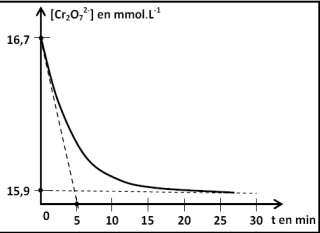
\includegraphics[width=0.5\textwidth]{./img/ex5.png}
  \end{center}
\end{wrapfigure}


Cette réaction est
lente, son évolution est suivie par dosage.

À la date $t = 0$, on mélange $V_p=2mL$ de sang prélevé au bras d’un conducteur avec $V= 10mL$ d’une solution aqueuse acidifiée de dichromate de potassium $(2K^+ + {Cr_2O_7^{2-}}_{(aq)})$ de concentration molaire $C=2.10^{-2} mol.L^{‐1}$.

Le volume total du mélange réactionnel est $V_M$=$12 mL$.

Un suivi temporel obtenu par dosage des ions dichromate $Cr_2O_7^{2-}$ a permis de tracer la courbe suivante.

\textbf{1. }Établir le tableau d’avancement du système en désignant par $n_0$ la quantité de matière initiale
d’alcool présente dans les $2mL$ de sang, et par $n_1$ la quantité de matière initiale en ions dichromate introduite dans le mélange réactionnel. (L’ion $H^+$ est en excès).

\textbf{2. }Quelle relation existe entre l’avancement x de la réaction, la concentration en ions dichromate $[Cr_2O_7^{2-}]$ dans le mélange, le volume $V_M$ du mélange réactionnel, et la quantité $n_1$ ?

\textbf{3. }La réaction peut être considérée comme
totale. À l’aide du graphique $[Cr_2O_7^{2-}]$ =$ f(t)$,
calculer l’avancement maximal.

\textbf{4. }Le taux autorisé d’alcool est de 0,5 g dans 1 L
de sang. Le conducteur est‐il en infraction ?

\textbf{5. }Donner la définition de la vitesse de la
réaction.

\textbf{6. }Déterminer sa valeur à l’instant initial.

\textbf{Données : Masse molaire moléculaire de l’éthanol 46g/mol}

\end{Box2}


\end{document}
